\documentclass[a4paper, 11pt, final, garamond]{book}
\usepackage{cours-preambule}

\makeatletter
\renewcommand{\@chapapp}{Devoir surveill\'e -- num\'ero}
\makeatother

\begin{document}
\setcounter{chapter}{7}

\def\lspace{25}

\chapter{Commentaires sur le DS n\degree08}
\section{Commentaires généraux}

Ça n'était pas un devoir surveillé compliqué, beaucoup de techniques classiques
et répétées, mais il est pourtant mal réussi. La moyenne est à 09/20. Revoyez
vraiment votre compréhension des réactions acide-base, il faut voir plus loin
que le cours et chercher des exercices en-dehors des TDs en cours pour changer
vos perspectives.

Au niveau des remarques du DS précédent, c'est globalement correct. \num{+0.5}
pour une remarque peu pertinente ou beaucoup partagée («~ne pas confondre
dimension et unité~» par exemple). Je ne vous demandais pas une remarque
pertinent pour le DS de chimie, mais une remarque pertinente vis-à-vis du DS
précédent. Je vous demanderai la même chose pour le suivant, mais \textbf{ne
	vous limitez pas à ce document}~: vous pouvez faire des remarques
\textbf{personnelles} sur votre DS précédent, qui sera plus récompensé en bonus.

Il y a eu plusieurs personnes qui ont repris un exercice ou problème plus loin
dans leur copie. \textbf{Aucune question reprise plus tard n'a été lue ou
	corrigée si la reprise n'a pas été indiquée en amont}. On ne m'amuse pas à
compter les points d'un problème et écrire le nombre de points pour devoir
revenir dessus plus tard parce que vous n'avez pas pris le temps de mettre une
astérisque.

Il est rédibitoire et très peu sérieux de confondre acide et base… Il faut
renseigner l'unité des potentiels que vous calculez~!

\begin{figure}[htbp!]
	\centering
	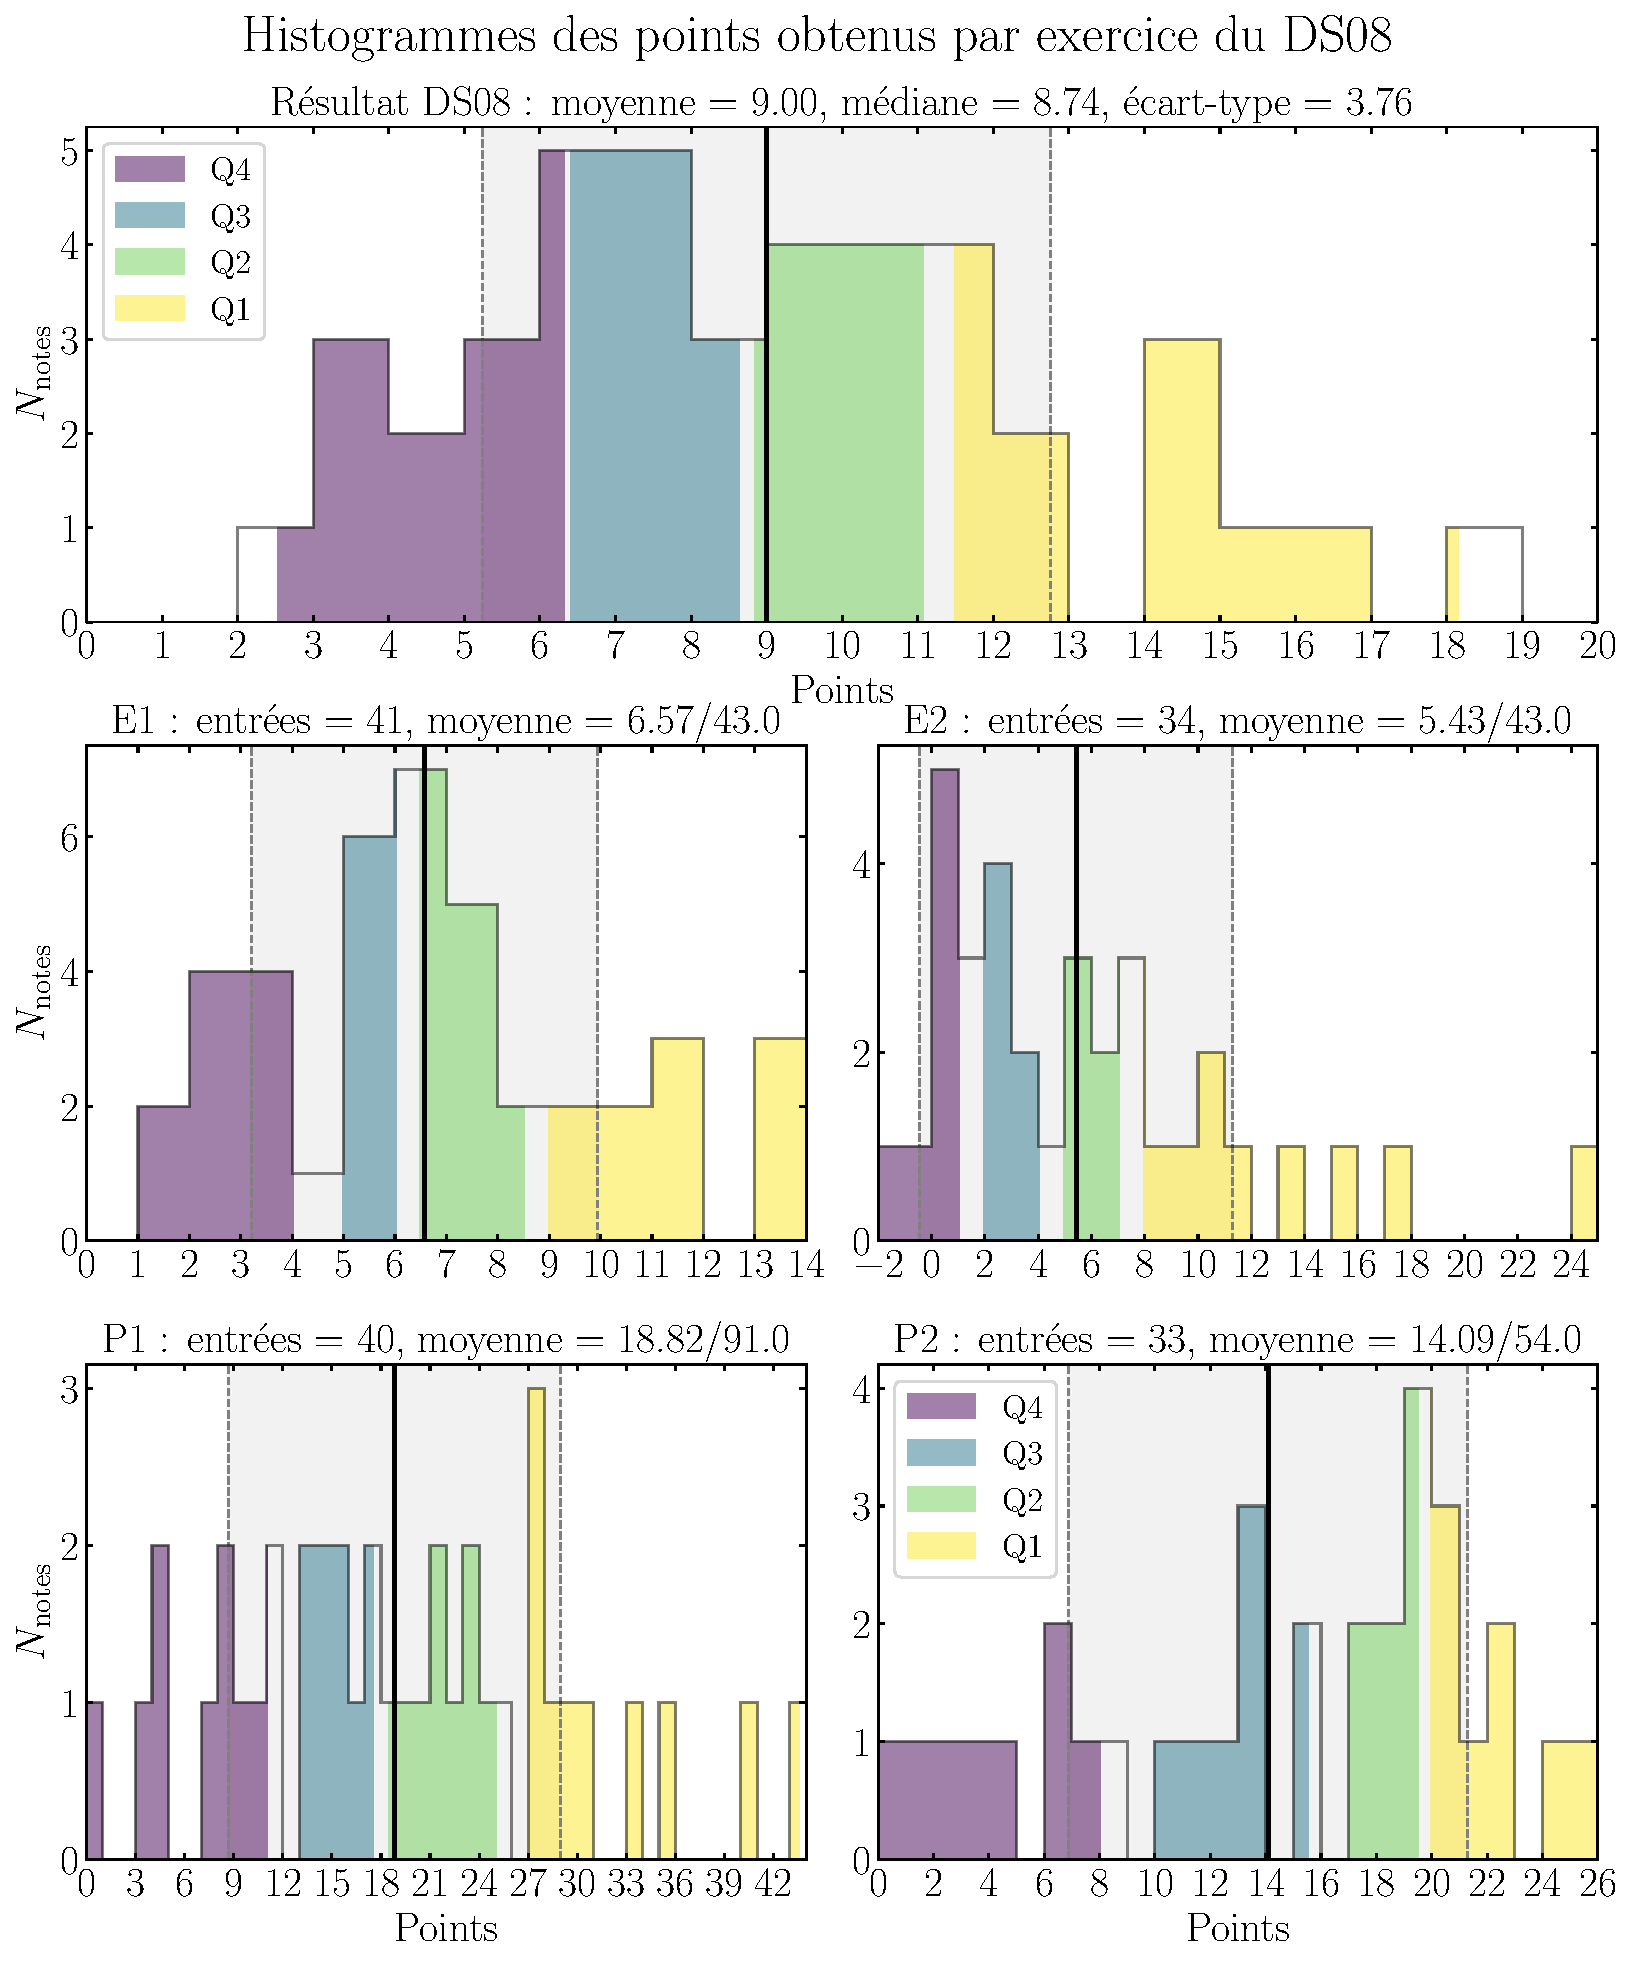
\includegraphics[width=1\linewidth]{DS08_hist_all}
\end{figure}

\setcounter{section}{0}
\section[43]"E"{Dioxyde de carbone en solution aqueuse}
Exercice très mal réussi. Revoyez la question 2 et la question 5, et pensez à la
\textbf{conservation de la matière}. Pléthore de résultats numériques absurdes,
même si souvent commentés comme tels, c'est bien.
\begin{enumerate}[label=\sqenumi]
	\item[n]{2}% Q1
	Bien~!
	\item[n]{10}% Q2
	Méthode élémentaire, dernière partie du cours acide-base, non maîtrisée.
	C'est fâcheux. \textbf{Faites des tableaux d'avancement}.
	\item[n]{3}% Q3
	Merci les calculatrices ! Plus sérieusement, l'architecture de la matière et
	le tableau périodique interviennent dans \textbf{tous les chapitres} et dans
	\textbf{toutes les épreuves} de concours.
	\item[n]{3}% Q4
	La cata. Méthode de décompte d'électrons et de doublet jamais entamée.
	Des cycles à 4 éléments complètement lunaires.
	\item[n]{7}% Q5
	Aïe. Même principe que question 2), l'idée des A/B n'est pas maîtrisée.
	\textbf{Quand on met un acide dans l'eau, il réagit}~! Si on met un acide à
	une certaine concentration initiale dans l'eau, sa concentration varie selon
	le $\pH$.
	\item[n]{2}% Q6
	Faites des schémas… Ça n'est \textbf{pas normal} de ne pas réussir à
	déterminer la composition d'une solution dont on vous écrit la composition
	en français~! Vous ne savez toujours pas ce qu'est la soude, et c'est grave.
	\item[n]{10}% Q7
	Attention, pour les réactions acide-base \textbf{il faut faire apparaître les
		couples},
	\item[n]{6}% Q8
	Idem.
\end{enumerate}

\section[43]"E"{Autour du chrome}
\begin{enumerate}[label=\sqenumi]
	\item[n]{2}% Q1
	Il faut justifier le caractère amphotère par des équations acide-base.
	\item[n]{3}% Q2
	\item[n]{2}% Q3
	Il faut savoir exploiter les diagrammes de solubilité.
	\item[n]{4}% Q4
	Définition de $K_s$~!
	\item[n]{6}% Q5
	Technique classique du cours, non maîtrisée.
	\item[n]{7}% Q6
	Si 5) réussie, 6) réussie. Par contre, \textbf{on ne peut pas comparer les
		solubilités sur la base du $K_s$}~! Ça dépend de la stœchiométrie.
	\item[n]{5}% Q7
	Celle du TP~!
	\item[n]{2}% Q8
	Pas mal. Vérifiez la règle de l'octet avec les DnL.
	\item[n]{2}% Q9
	pH = électrode de verre pour la mesure, référence au calomel saturée.
	\item[n]{2}% Q10
	Attention, pour les réaction acide-base \textbf{il faut faire apparaître les
		couples}, c'est-à-dire ici $\ce{H_2O/HO^-}$~!
	\item[n]{3}% Q11
	Attention à la stœchiométrie des équivalences~!
	\item[n]{5}% Q12
	Technique de demi-équivalence très utile à retenir.
\end{enumerate}

\setcounter{section}{0}
\section[88]"P"{Propriétés de l'azote}
\begin{enumerate}[label=\sqenumi]
	\item[n]{2}% Q1
	\textbf{1 mole de diazote} est une manière particulière de dire
	\textbf{coefficient stœchiométrique de 1} devant \ce{N2}.
	\item[n]{4}% Q2
	N'oubliez jamais la source initiale du quotient réactionnel~! Il faut
	connaître les activités et la \textbf{loi de \textsc{Dalton}} pour les gaz~!
	\item[n]{2}% Q3
	Idem.
	\item[n]{2}% Q4
	On applique ici les techniques de vraisemblance pour comprendre comment une
	valeur varie en fonction des variables littérales. Ce sont vraiment des
	techniques nécessaires à tout-e bon-ne scientifique. Si $Q \searrow$, alors $Q
		< K^\circ$ donc on retourne en sens direct~!
	\item[n]{1}% Q5
	RAS.
	\item[n]{7}% Q6
	Établir les doublets est \textbf{nécessaire} pour les schémas de
	\textsc{Lewis}~! Vérifiez l'octet. \textbf{Il y a 2 écarts à l'octet~:
		l'hypervalence et l'électrodéficience}. Les éléments de la \textbf{deuxième
		période} \textbf{ne peuvent être hypervalents}.
	\item[n]{2}% Q7
	RAS.
	\item[n]{2}% Q8
	Redoublez d'attention pour les équations rédox, faites un décompte de chaque
	élément et des charges. Mauvaise équation $\Ra$ mauvais tout ensuite.
	\item[n]{5}% Q9
	Revoir le principe de stabilité d'un mélange. Faites des échelles et/ou des
	diagrammes de prédominance.
	\item[n]{4}% Q10
	Globalement bien.
	\item[n]{2}% Q11
	RAS.
	\item[n]{4}% Q12
	\item[n]{2}% Q13
	Bien.
	\item[n]{2}% Q14
	RAS.
	\item[n]{2}% Q15
	\textbf{Hydroxyde de sodium} en solution donne $(\ce{Na^+}~;~\ce{HO^-})$, et
	ce sont les ions hydroxydes qui nous intéressent.
	\item[n]{3}% Q16
	Bien.
	\item[n]{3}% Q17
	\item[n]{4}% Q18
	\item[n]{7}% Q19
	Il faut savoir conclure, et surtout quand est-ce qu'on ne peut pas
	conclure~! Pas d'incertitude $\Ra$ valeur faiblement comparable.
	\item[n]{2}% Q20
	Bien~!
	\item[n]{9}% Q21
	Technique de calcul de $K^\circ$ redox globalement maîtrisée, bravo !
	\item[n]{3}% Q22
	Manque d'analyse, refaites des schémas. Presque similaire au TP24 sur le
	dosage indirect, ne négligez pas l'importance des TP et leur préparation.
	\item[n]{3}% Q23
	Rien de plus classique que ce dosage.
	\item[n]{4}% Q24
	RAS.
	\item[n]{3}% Q25
	RAS.
	\item[n]{4}% Q26
	RAS.
\end{enumerate}

\section[53]"P"{$E-\pH$ du chlore}
\begin{enumerate}[label=\sqenumi]
	\item[n]{7}% Q1
	Très bien~! Le remplissage des espèces est qualitatif et méthodique. Par
	contre, c'est $\no{Cl \in Cl_2}$~! $\no{Cl_2}$ n'a pas de sens.
	\item[n]{3}% Q2
	Retravaillez l'exploitation des $E-\pH$ pour déterminer des constantes grâce
	aux frontières. \textbf{Ne confondez pas $\pH$ et $\pH\ind{front}$}.
	\item[n]{7}% Q3
	Manque d'analyse et de compréhension générale de l'utilisation des
	frontières. Vous pensez que les $E^\circ$ sont sur les frontières, mais
	$E\ind{front} \neq E^\circ$~! Il faut \textbf{écrire la demi-équation}, puis
	la \textbf{formule de \textsc{Nernst}}, et enfin \textbf{déterminer
		$E\ind{front}$} et en conclure la valeur de $E^\circ$. \xul{Vous ne pouvez pas
		lire des $E^\circ$ sur un $E-\pH$}.
	\item[n]{9}% Q4
	RAS.
	\item[n]{3}% Q5
	Il faut vraiment savoir lire n'importe quel graphique et relier des
	coordonnées à une donnée exploitatble. En toute rigueur, \textbf{une pente a
		une unité}, ici des \si{V/\pH}. Vous ne pouvez pas dire «~la vérification
	graphique valide la valeur~» sans expliquer la vérification, en
	\textbf{encore moins} quand votre valeur est fausse…
	\item[n]{9}% Q6
	Idem.
	\item[n]{8}% Q7
	Trop d'erreus d'équilibrage. \textbf{«~Par le cours~» n'est jamais un
		argument recevable}. Vous êtes des scientifiques, vous n'invoquez pas un
	cours, remplacez par «~On sait que~» (si c'est en effet évident).
	\item[n]{4}% Q8
	Conclusion sur stabilité avec l'eau OK, manque manque d'argument (domaines
	disjoints).
	\item[n]{4}% Q9
	Anode = oxydation, cathode = réduction.
	\item[n]{4}% Q10
	Bien sur la dismutation ici aussi.
	\item[n]{9}% Q11
	Correct, il faut savoir extraire les bonnes valeurs de l'énoncé.
	\item[n]{4}% Q12
	Manque de compréhension entre électrons transmis et intensité.
	\item[n]{3}% Q13
	Entraînez-vous à commenter des résultats~!
\end{enumerate}

\end{document}
